\section{Casos de uso}
El la siguiente seccion se define y describen los esenarios entre los actores y ARF describiendo las entidades de negocio y su funcionalidad dentro de la aplicación, así mismo su interacción con los actores interesados con la aplicación.\par
\begin{figure}[h!]
	\centering
	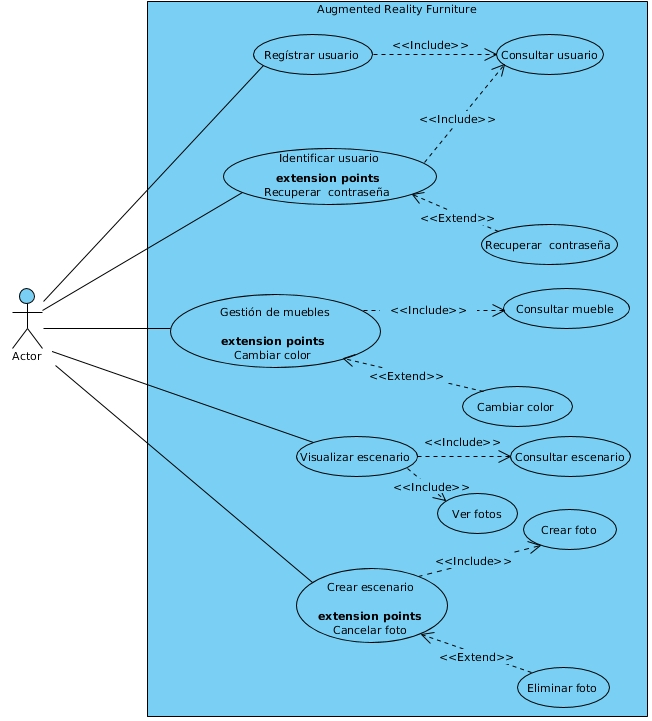
\includegraphics[width=13cm,height=15cm]{imagenes/analisis/casosDeUso.jpg}
	\caption{Casos de uso del usuario.}
	\label{fig:analogo}
\end{figure}  
\newpage

\subsection{Actores}
\textbf{Nombre del actor:} \textit{Cliente} \textbf{(Usuario)}\par
\textbf{Definición :} Usuario final y el principal interesado en usar nuestra aplicación. Tendrá los permisos de un usuario estándar, este actor sera el único considerado hasta este momento ya que en iteraciones posteriores se contempla el aumento de usuarios. A continuación se describen las funciones donde interviene la aplicación este usuario.

\subsection{Login}
\begin{figure}[h!]
	\centering
	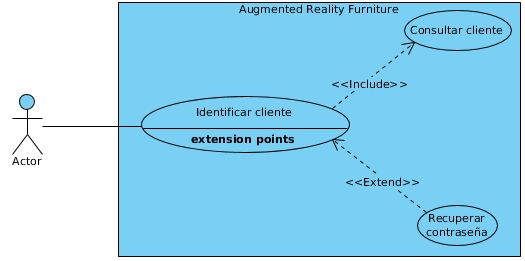
\includegraphics[width=9cm,height=5cm]{imagenes/analisis/login.jpg}
	\caption{CU01 Login.}
	\label{fig:analogo}
\end{figure}  

\subsection{Registrar usuario} 
\vspace{5mm} 	
\begin{figure}[h!]
	\centering
	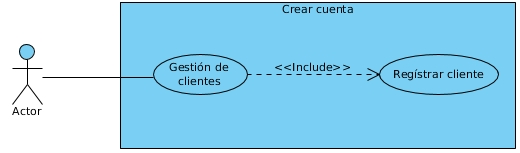
\includegraphics[width=10cm,height=3cm]{imagenes/analisis/registro.jpg}
	\caption{CU02 Registrar un usuario.}
	\label{fig:analogo}
\end{figure} 
\newpage
\subsection{Seleccionar mueble} 
\vspace{5mm}
\begin{figure}[h!]
	\centering
	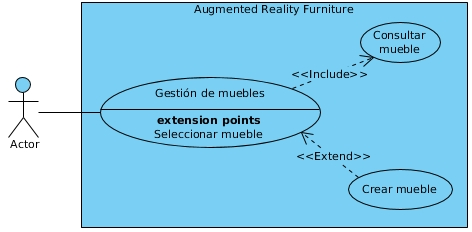
\includegraphics[width=9cm,height=4cm]{imagenes/analisis/seleccionarMueble.jpg}
	\caption{CU3 Seleccionar mueble.}
	\label{fig:analogo}
\end{figure}

\subsection{Gestión de escenario} 
\vspace{5mm}
\begin{figure}[h!]
	\centering
	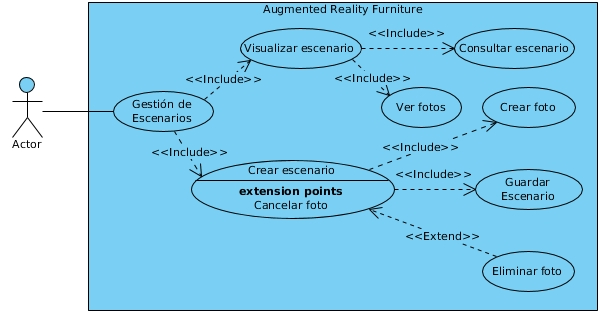
\includegraphics[width=12cm,height=6cm]{imagenes/analisis/gestionEscenarios.jpg}
	\caption{CU04 Gestionar escenario.}
	\label{fig:analogo}
\end{figure}
